\begin{appendices}

\chapter{Manual técnico}\label{anexo:manual_tecnico}

El presente manual técnico detalla el procedimiento para la clonación, configuración de dependencias, puesta en marcha del entorno de desarrollo local y reproducción íntegra de la batería de pruebas y análisis de rendimiento del sistema.

\section{Requisitos previos del sistema}\label{sec:manual_requisitos}

Para garantizar la correcta ejecución de la plataforma en un entorno local, la máquina anfitriona debe disponer de las herramientas base instaladas y registradas en las variables de entorno del sistema (\texttt{PATH}):

\begin{itemize}
    \item \textbf{Git}\cite{git_official}.
    \item \textbf{Node.js}\cite{nodejs_official}.
    \item \textbf{\texttt{uv}}\cite{uv_official} (puede instalarse nativamente o mediante \texttt{pip} si el sistema ya cuenta con un intérprete de Python).
\end{itemize}

\section{Preparación y configuración del repositorio}\label{sec:manual_preparacion}

\subsection*{Descarga del código fuente}
Clonar el repositorio del proyecto e ingresar en el directorio raíz:

\begin{lstlisting}
(*@\cliPrompt@*) (*@\bashYellow{git}@*) clone https://github.com/frangago71/quizzie-TFG.git
(*@\cliPrompt@*) (*@\bashYellow{cd}@*) quizzie-TFG
\end{lstlisting}

\subsection*{Configuración del entorno del backend}
Instalar el gestor \texttt{uv} en caso de no disponer de él previamente y sincronizar todas las dependencias del proyecto:

\begin{lstlisting}
(*@\cliPrompt@*) (*@\bashYellow{pip}@*) install uv
(*@\cliPrompt@*) (*@\bashYellow{uv}@*) sync (*@\bashGrey{--all-groups}@*)
\end{lstlisting}

La sincronización anterior genera un entorno virtual aislado (\texttt{.venv}) con todas las librerías necesarias. Para la ejecución de órdenes en dicho entorno se puede emplear el prefijo \texttt{uv run} en cada invocación, o bien activar explícitamente el entorno en la sesión de terminal para omitir dicho prefijo y ejecutar los comandos directamente:

\begin{lstlisting}
(*@\cliPrompt@*) (*@\bashYellow{\&}@*) .\.venv\Scripts\Activate.ps1
\end{lstlisting}

Para poblar la base de datos con los registros iniciales, acceder al directorio del backend y ejecutar el script de sembrado:

\begin{lstlisting}
(*@\cliPrompt@*) (*@\bashYellow{cd}@*) backend
(*@\cliPrompt@*) (*@\bashYellow{uv}@*) run python -m seed            (*@\covGreen{\# Ejecutar el sembrado inicial de datos}@*)
\end{lstlisting}

\subsection*{Configuración del entorno del frontend}
Acceder al directorio de la interfaz de usuario e instalar los módulos de dependencias:

\begin{lstlisting}
(*@\cliPrompt@*) (*@\bashYellow{cd}@*) ../frontend
(*@\cliPrompt@*) (*@\bashYellow{npm}@*) install                          (*@\covGreen{\# Instalar dependencias de Node.js}@*)
\end{lstlisting}

\subsection*{Configuración de variables de entorno}\label{subsec:manual_env}
Copiar la plantilla de configuración situada en la raíz del proyecto para generar el archivo local \texttt{.env}:

\begin{lstlisting}
(*@\cliPrompt@*) (*@\bashYellow{cp}@*) .env.example .env
\end{lstlisting}

A continuación, editar el archivo \texttt{.env} completando las siguientes secciones:

\begin{itemize}
    \item \textbf{\texttt{VITE\_API\_URL}}: Dirección base donde escucha la API de FastAPI. En local se establece en \texttt{http://localhost:8000}; en producción apuntará a la URL del backend desplegado.
    \item \textbf{\texttt{SECRET\_KEY}}: Clave simétrica utilizada para firmar criptográficamente los tokens de sesión. Para garantizar la seguridad, se recomienda generarla de manera aleatoria, por ejemplo ejecutando el siguiente comando en la terminal:
\begin{lstlisting}
(*@\cliPrompt@*) (*@\bashYellow{openssl}@*) rand -hex 32
\end{lstlisting}
    \item \textbf{\texttt{ALGORITHM}}: Algoritmo criptográfico de firma de tokens (por defecto, \texttt{HS256}).
    \item \textbf{\texttt{ACCESS\_TOKEN\_EXPIRE\_MINUTES}}: Tiempo de expiración del token de sesión expresado en minutos (fijado por defecto en 30).
    \item \textbf{\texttt{SMTP\_HOST}}: Nombre de dominio del servidor de correo saliente (por defecto, \texttt{smtp.gmail.com}).
    \item \textbf{\texttt{SMTP\_PORT}}: Puerto del servicio de transporte. Los valores habituales son \texttt{465} (cifrado implícito SSL) o \texttt{587} (cifrado explícito TLS/STARTTLS).
    \item \textbf{\texttt{SMTP\_USERNAME}}: Cuenta de correo electrónico empleada para la autenticación ante el servidor SMTP.
    \item \textbf{\texttt{SMTP\_PASSWORD}}: Clave de acceso al servicio. Al emplear Gmail, es indispensable utilizar una \textbf{Contraseña de aplicación} de Google generada desde la cuenta de seguridad, en lugar de la contraseña principal de usuario.
    \item \textbf{\texttt{SMTP\_FROM}}: Dirección visible en la cabecera del remitente. Si se omite, toma automáticamente el valor de \texttt{SMTP\_USERNAME}. En servidores como Gmail, este campo debe coincidir con la cuenta autenticada para evitar que el servidor rechace el envío por sospecha de suplantación.
    \item \textbf{\texttt{GEMINI\_API\_KEY}}: Clave de acceso a la API de Google Gemini para la generación asistida de cuestionarios. Corresponde a una funcionalidad planificada para la siguiente etapa y que queda fuera del alcance de la presente entrega del TFG.
\end{itemize}

El archivo \texttt{.env} resultante se encuentra excluido mediante el archivo \texttt{.gitignore}, garantizando que ninguna credencial privada alcance el repositorio remoto.

\section{Ejecución del proyecto en el entorno local}\label{sec:manual_ejecucion}

La plataforma requiere la ejecución simultánea de dos procesos independientes. Para ello, se recomienda disponer de dos terminales de trabajo activas de manera concurrente.

\subsection*{Terminal 1: Servicio del backend (FastAPI)}
Iniciar el servidor de desarrollo del \textit{backend}:

\begin{lstlisting}
(*@\cliPrompt@*) (*@\bashYellow{cd}@*) backend
(*@\cliPrompt@*) (*@\bashYellow{uv}@*) run fastapi dev        
\end{lstlisting}

Una vez levantado el servicio, los accesos locales quedan disponibles en:
\begin{itemize}
    \item \texttt{http://127.0.0.1:8000}: Raíz del servidor y servicio de la API.
    \item \texttt{http://127.0.0.1:8000/docs}: Documentación - \textbf{Swagger UI}.
    \item \texttt{http://127.0.0.1:8000/redoc}: Documentación - \textbf{ReDoc}.
\end{itemize}

\subsection*{Terminal 2: Cliente del frontend (Vite)}
Acceder al directorio de la interfaz y levantar el servidor de desarrollo local:

\begin{lstlisting}
(*@\cliPrompt@*) (*@\bashYellow{cd}@*) frontend
(*@\cliPrompt@*) (*@\bashYellow{npm}@*) run dev               
\end{lstlisting}

La interfaz web quedará accesible desde el navegador en \texttt{http://localhost:5173}.

\section{Procedimiento de ejecución de pruebas y cobertura}\label{sec:manual_pruebas}

\subsection*{Pruebas unitarias y de integración del \textit{backend}}

Ejecutar la suite completa de pruebas unitarias y de integración del \textit{backend} mediante \texttt{pytest}:

\begin{lstlisting}
(*@\cliPrompt@*) (*@\bashYellow{uv}@*) run pytest
\end{lstlisting}

Para auditar la cobertura de código y generar reportes adicionales, se pueden combinar los siguientes modificadores:

\begin{itemize}
    \item \texttt{--cov=backend}: Delimita el análisis exclusivamente al código fuente del \textit{backend}.
    \item \texttt{--cov-report=term-missing}: Imprime en la consola la tabla desglosada por módulo señalando las líneas exactas sin cobertura.
    \item \texttt{--cov-report=html}: Genera un informe visual interactivo estructurado dentro del directorio local \texttt{htmlcov/}.
\end{itemize}

Al combinar estas tres opciones, se imprime en la terminal la tabla de cobertura del \textit{backend} y se genera un informe interactivo en \texttt{htmlcov/index.html}:

\begin{lstlisting}
(*@\cliPrompt@*) (*@\bashYellow{uv}@*) run pytest (*@\bashGrey{--cov=backend --cov-report=term-missing --cov-report=html}@*)
\end{lstlisting}

\begin{evidence}[H]
    \centering
    \makebox[\textwidth][c]{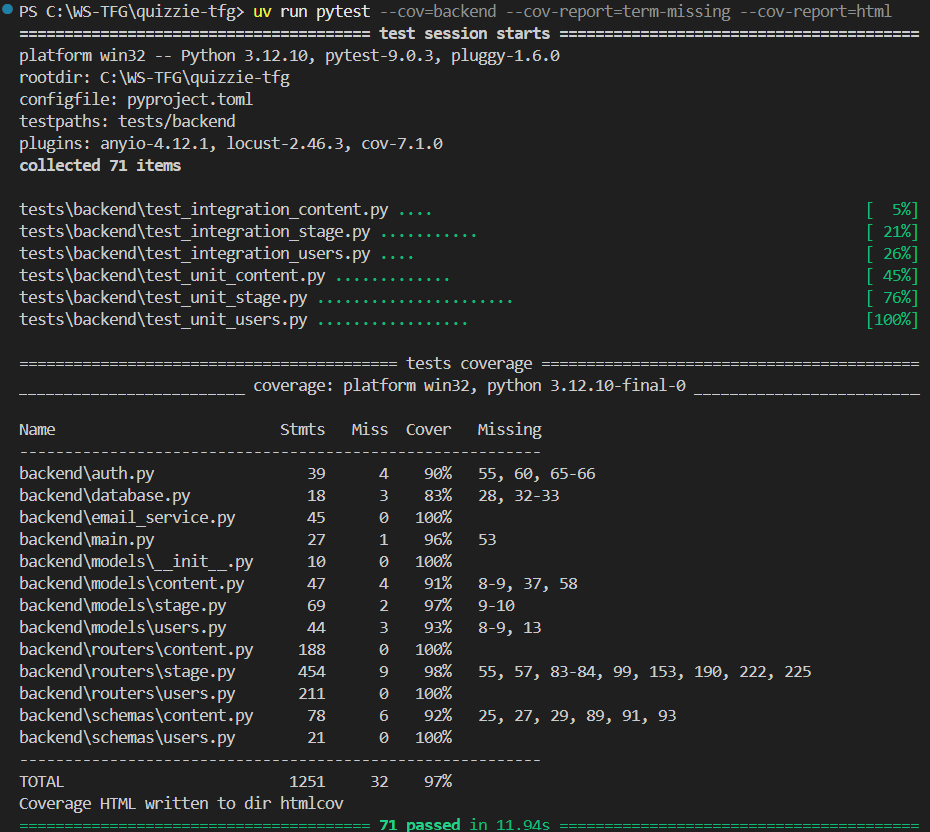
\includegraphics[width=0.82\textwidth]{evidences/terminal_test_backend.png}}
    \captionsetup{hypcap=false}
    \caption*{Salida por terminal al ejecutar las pruebas y la cobertura del \textit{backend}.}
\end{evidence}

Para abrir el reporte web directamente en el navegador predeterminado desde la consola según el sistema operativo:

\begin{lstlisting}
(*@\cliPrompt@*) (*@\bashYellow{start}@*) htmlcov/index.html                  (*@\covGreen{\# Windows}@*)
(*@\cliPrompt@*) (*@\bashYellow{xdg-open}@*) htmlcov/index.html                 (*@\covGreen{\# Linux}@*)
(*@\cliPrompt@*) (*@\bashYellow{open}@*) htmlcov/index.html                     (*@\covGreen{\# macOS}@*)
\end{lstlisting}

De manera alternativa, el informe puede consultarse abriendo el archivo a través del explorador del sistema operativo.

\subsection*{Pruebas de componentes del \textit{frontend}}

Acceder al directorio de la interfaz y ejecutar la suite completa de pruebas unitarias y de componentes:

\begin{lstlisting}
(*@\cliPrompt@*) (*@\bashYellow{cd}@*) frontend
(*@\cliPrompt@*) (*@\bashYellow{npm}@*) run test
\end{lstlisting}

Ejecutar la suite de pruebas evaluando la cobertura de código:

\begin{lstlisting}
(*@\cliPrompt@*) (*@\bashYellow{npm}@*) run test:frontend:coverage
\end{lstlisting}

Al ejecutar este comando, se imprime por terminal el desglose cuantitativo de cobertura acotado a los módulos clave (\texttt{auth}, \texttt{management}, \texttt{room-access} y \texttt{room-play}) y se genera el directorio de cobertura \texttt{frontend/coverage/}:

\begin{evidence}[H]
    \centering
    \makebox[\textwidth][c]{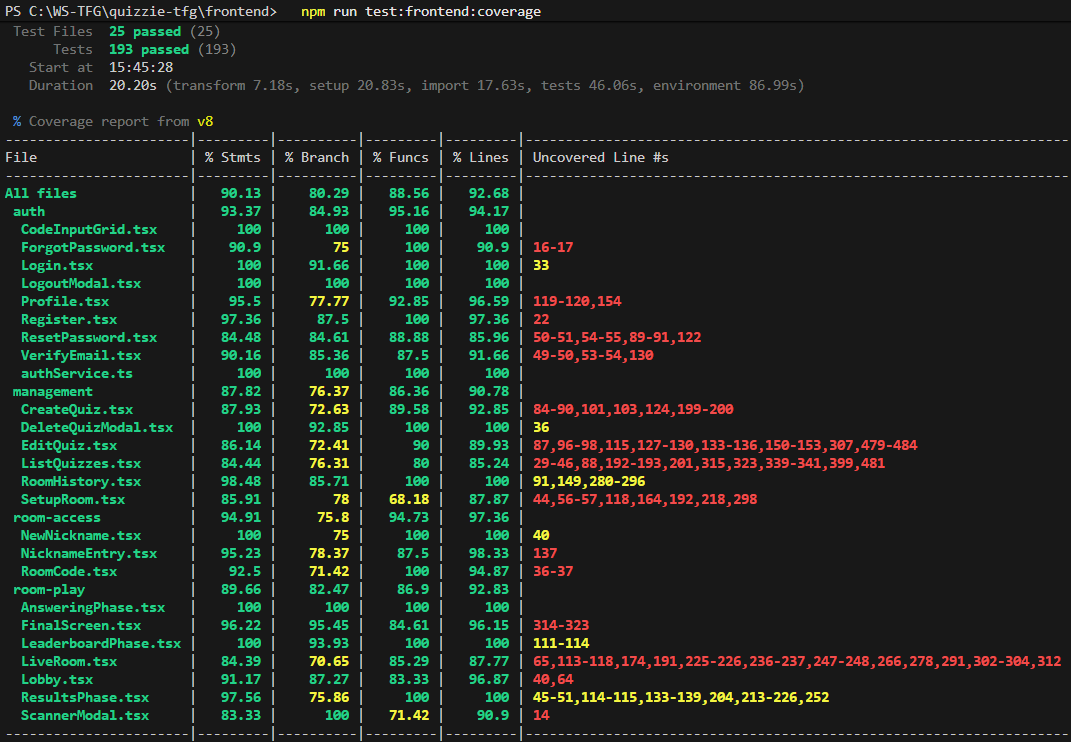
\includegraphics[width=\textwidth]{evidences/terminal_test_componentes.png}}
    \captionsetup{hypcap=false}
    \caption*{Salida por terminal al ejecutar las pruebas y la cobertura de componentes.}
\end{evidence}

Para visualizar en el navegador el informe web interactivo generado, iniciar el servidor local de visualización:

\begin{lstlisting}
(*@\cliPrompt@*) (*@\bashYellow{npm}@*) run cov-report:frontend
\end{lstlisting}

El reporte web queda desplegado en \texttt{http://localhost:4173}. Asimismo, es posible visualizarlo de forma estática cargando \texttt{frontend/coverage/index.html} en el navegador.

\subsection*{Pruebas de extremo a extremo y cobertura E2E}

Ejecutar la suite de pruebas \textit{End-to-End} sobre la compilación de producción del cliente web:

\begin{lstlisting}
(*@\cliPrompt@*) (*@\bashYellow{cd}@*) frontend
(*@\cliPrompt@*) (*@\bashYellow{npm}@*) run test:e2e
\end{lstlisting}

Al finalizar la ejecución, la consola muestra el resumen de los escenarios evaluados y se generan los informes de trazas de ejecución de casos de uso y de cobertura:

\begin{evidence}[H]
    \centering
    \makebox[\textwidth][c]{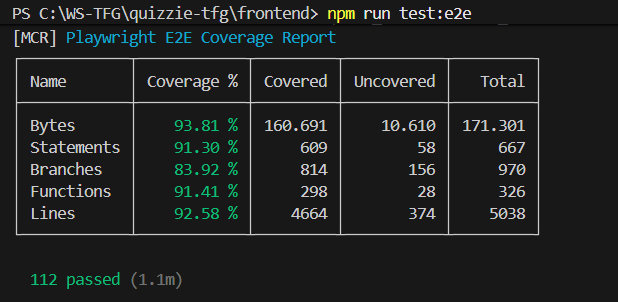
\includegraphics[width=0.85\textwidth]{evidences/terminal_test_e2e.png}}
    \captionsetup{hypcap=false}
    \caption*{Salida por terminal al ejecutar las pruebas de extremo a extremo.}
\end{evidence}

Para inspeccionar las trazas detalladas, capturas de pantalla y pasos de ejecución mediante el servidor integrado de Playwright:

\begin{lstlisting}
(*@\cliPrompt@*) (*@\bashYellow{npx}@*) playwright show-report
\end{lstlisting}

El reporte queda desplegado en \texttt{http://localhost:9323}, permaneciendo almacenado como archivo estático en \texttt{frontend/playwright-report/index.html}.

Para previsualizar el informe de cobertura interactivo generado por \textbf{Monocart}, levantar el servidor local:

\begin{lstlisting}
(*@\cliPrompt@*) (*@\bashYellow{npm}@*) run cov-report:e2e
\end{lstlisting}

El reporte queda accesible en \texttt{http://localhost:4174}, o bien abriendo directamente el archivo \texttt{frontend/coverage-e2e/index.html}.

\subsection*{Pruebas de carga y rendimiento}

Para ejecutar estas pruebas es necesario disponer de dos terminales abiertas: una manteniendo el servicio del \textit{backend} en ejecución en \texttt{http://127.0.0.1:8000} y otra situada en la raíz del proyecto para lanzar las pruebas.

El flujo de trabajo se compone de dos fases: en primer lugar, se inyecta la carga en el servidor mediante Locust, lo que genera automáticamente los registros de métricas en formato CSV dentro del directorio \texttt{tests/locust/}. Posteriormente, el script \texttt{tests/locust/evaluate\_thresholds.py} procesa dichos ficheros para verificar si los tiempos de respuesta y las tasas de error se mantienen dentro de los umbrales de aceptación definidos.

Para llevar a cabo la inyección de carga se dispone de dos alternativas válidas:

\subsubsection*{Opción 1: Modo interactivo con interfaz web}

Iniciar el panel gráfico de control de Locust para configurar los parámetros manualmente y monitorizar la prueba en tiempo real en \texttt{http://localhost:8089}:

\begin{lstlisting}[basicstyle=\fontsize{11.5pt}{13.2pt}\ttfamily\color{black}, aboveskip=4pt, belowskip=4pt]
(*@\cliPrompt@*) (*@\bashYellow{uv}@*) run locust -f tests/locust/locustfile.py --host http://127.0.0.1:8000
\end{lstlisting}

\subsubsection*{Opción 2: Ejecución por consola}

Ejecutar las pruebas directamente desde la terminal utilizando el script automatizado con la configuración base (200 usuarios, tasa de 15~u/s y 1~minuto de duración):

\begin{lstlisting}
(*@\cliPrompt@*) (*@\bashYellow{uv}@*) run python tests/locust/run_performance_tests.py
\end{lstlisting}

Para personalizar las condiciones de estrés, es posible sobrescribir estos valores mediante los siguientes argumentos:

\begin{lstlisting}
(*@\cliPrompt@*) (*@\bashYellow{uv}@*) run python tests/locust/run_performance_tests.py (*@\bashGrey{-u}@*) 300 (*@\bashGrey{-r}@*) 25 (*@\bashGrey{-t}@*) 2m
\end{lstlisting}

\begin{itemize}
    \item \texttt{-u} (\texttt{--users}): Número de usuarios virtuales simultáneos.
    \item \texttt{-r} (\texttt{--spawn-rate}): Tasa de incorporación de nuevos usuarios por segundo.
    \item \texttt{-t} (\texttt{--run-time}): Duración total de la prueba.
    \item \texttt{--host}: Dirección base del servicio \textit{backend}.
\end{itemize}

Una vez concluida la prueba mediante cualquiera de las dos alternativas y generados los archivos CSV, ejecutar el script de auditoría para verificar cuantitativamente el cumplimiento de los umbrales de aceptación:

\begin{lstlisting}
(*@\cliPrompt@*) (*@\bashYellow{uv}@*) run python tests/locust/evaluate_thresholds.py
\end{lstlisting}

\newpage

Al procesar los registros, la herramienta contrasta las latencias y tasas de error frente a los límites admisibles:

\begin{evidence}[H]
    \centering
    \makebox[\textwidth][c]{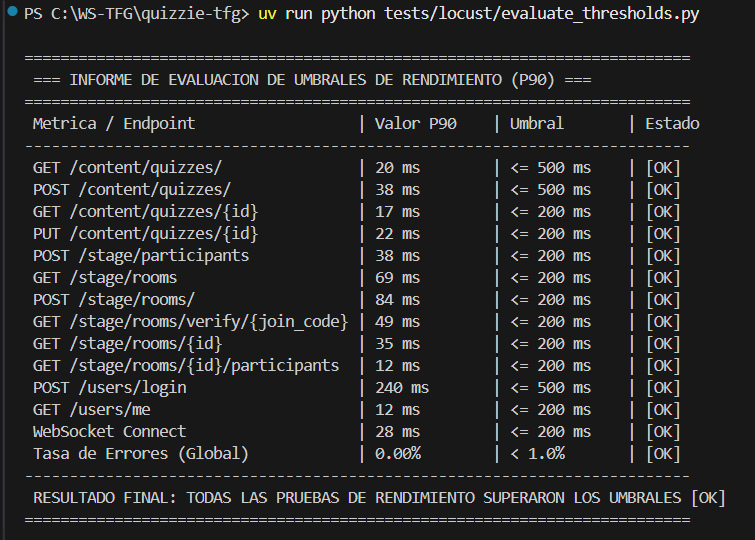
\includegraphics[width=0.85\textwidth]{evidences/terminal_test_umbrales.png}}
    \captionsetup{hypcap=false}
    \caption*{Salida por terminal del \textit{script} de cumplimiento de umbrales.}
\end{evidence}

\end{appendices}